        \documentclass{standalone}
        \usepackage{tikz}
        \usepackage{amsmath}
        \begin{document}
        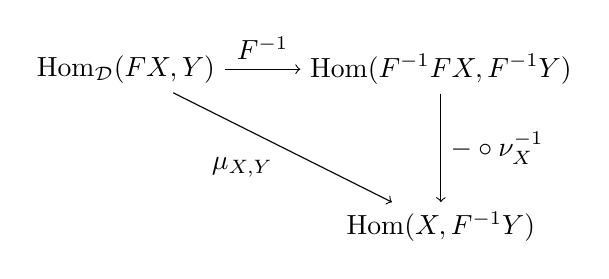
\begin{tikzpicture}

        \node at (0,0) (F) {$\operatorname{Hom}_{\mathcal D}(FX,Y)$};
        \node at (4,0) (Finv) {$\operatorname{Hom}(F^{-1}FX,F^{-1}Y)$};
        \node at (4,-2) (E) {$\operatorname{Hom}(X,F^{-1}Y)$};
        \draw[->] (F) -- node[above] {$F^{-1}$} (Finv);
        \draw[->] (Finv) -- node[right] {$- \circ \nu_X^{-1}$} (E);
        \draw[->] (F) -- node[below left] {$\mu_{X,Y}$} (E);
            \end{tikzpicture}
        \end{document}
